\section{Design}
\label{sec:design}
Our design is built of relatively large submodules, so that not many additional elements are necessary in the top module. The structure can be seen in Fig. \ref{fig:processoroverview}. The main modules are the instruction decoder, the register file, the ALU, the memory interface and the instruction fetch module. These modules are described in detail in the following sections.

\begin{figure}[ht]
\centering
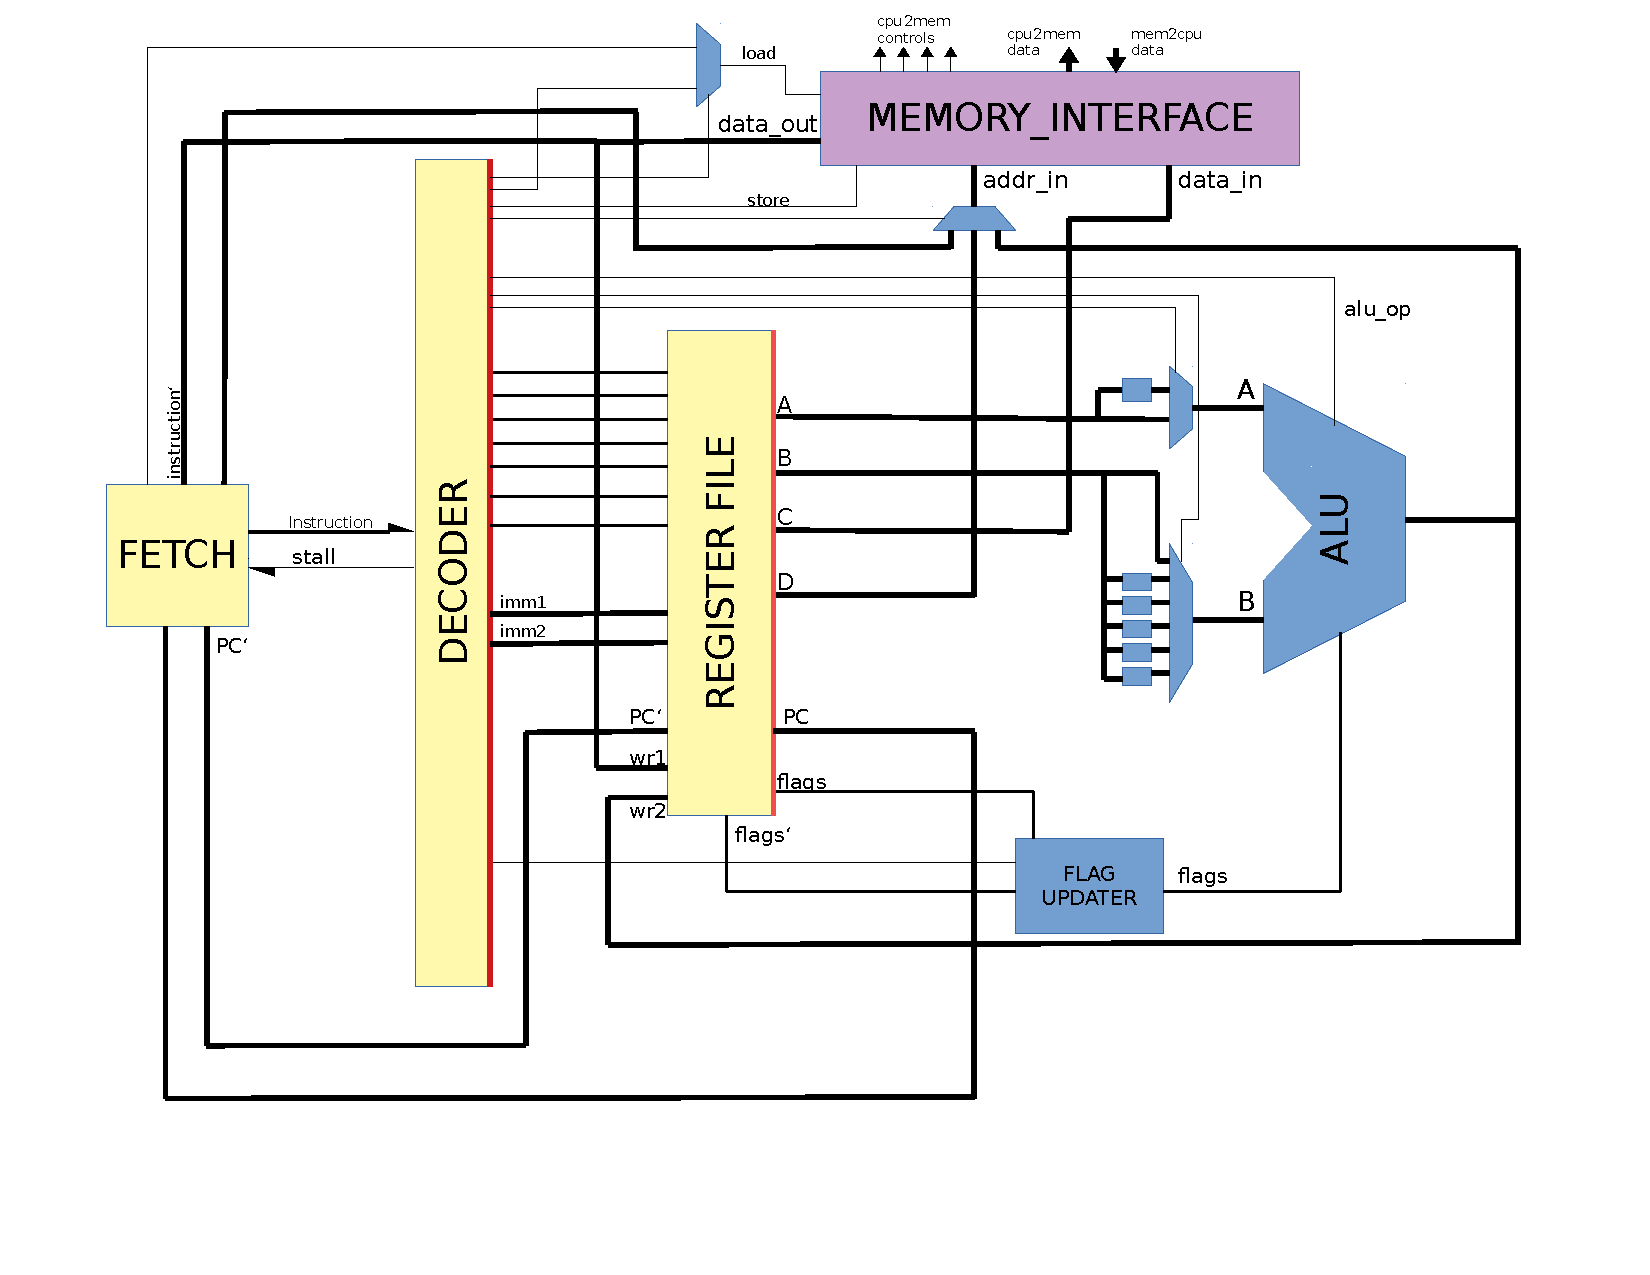
\includegraphics[scale=0.65]{images/processorOverview.pdf}
\caption{The block structure of the processor design. Register stages are marked red.}
\label{fig:processoroverview}
\end{figure}

In the block structure, the modules are connected with several connections, but only the address and load inputs for the memory are busses with more than one input. All other connections can only be driven by one module, which simplifies the overall structure. 

\subsection{Processor Control}
\label{subsec:processorcontrol}
The control of the execution and memory access is performed by a state machine in the decoder module. Initially, a dedicated controller for the memory access and pipeline stalls was planned; while integrating and testing the decoder, the function of the controller was integrated into the decoder. It yet had many control functions in order to perform multi-cycle instruction like \texttt{MULTI-PUSH/-POP}.

Almost all control signals are outputs of the decoder. These include the ALU opcode, register selects, the flag updates and memory access signals. As the memory access must be arbitrated, the instruction fetch controls the multiplexors assigning the read request and address signals from itself and the decoder module. When the current instruction accesses the memory, a stall signal to the instruction fetch can be set by the decoder. On the other hand, the instruction fetch may stall the decoder (which then stalls the rest of the processor) if the next instruction is not loaded yet. With this mechanisms, we tried to keep the control of the processor as simple as possible.

\subsection{Pipeline Stages}
\label{subsec:pipelinestages}

Our processor is comprised of two pipeline stages. One stage includes the instruction fetch and decoder, the other one does the execution and writeback tasks. These two stages have been chosen because of the structure of the benchmark applications and the 1-port memory. The applications are both relatively memory-access-loaded. The memory allows only one access per cycle; additionally, it is halfword-aligned, while the architecture uses byte-aligned addresses. The benchmarks both frequently access whole words in the memory, so that in many cycles, the memory would be the bottleneck in the execution. With only two pipeline stages, few stalls would occur. 

\subsection{Modules}
\label{subsec:modules}
In the following, an insight view into the single modules' implementation is given.

\subsubsection{ALU}
\label{subsubsec:alu}
The arithmetic logic unit (ALU) performs the calculations stated in the instructions.\\
Its 32-bit structure is purely combinatorial. All logical and arithmetical operations defined in chapter 5.4.1 in the THUMB instruction set (\textbf{TODO} are supported. Each computation can be executed within a single clock cycle.\\
\newline
Which operation to perform by the ALU is decided by the 4-bit opcode from the instruction fetch. This determines also if along the two signed input signals the input carry flag is needed.\\
The result consists of a 32-bit signed output value, as well as the four condition code flags negative (n), zero (z), carry (c) and overflow (v). Depending on the computed instruction, the application program status register (APSR) in the register file gets updated by the Flag Updater with those flags.


\subsubsection{Instruction Fetch}
\label{subsubsec:instructionfetch}
The instruction fetch (IF) is used for loading new instructions from the memory and passing them to the instruction decoder.\\
The module itself is build as a finite state machine and consists of four separate states. One of them is for reset, two are working states (wait and fetch) and the last one is entered when the executed program is finished.\\
\newline
At the startup, the decoder does not posses any instruction to perform, so the IF begins in fetch state. To get the first instruction, an address, which is two less than the current value of the program counter (PC), and a load request is sent to the memory interface.\\
When the wanted data arrives back, it gets passed to the decoder for one clock cycle. Furthermore the PC gets incremented by two, which matches the length of one instruction, 16 bit. The IF switches to wait state.\\
As long as the decoder is executing the new instruction, the IF gets stalled and remains in its current state. When finished, the instruction fetch switches back to fetch state again and starts to load the next instruction.\\
When the last instruction got performed, the instruction fetch switches to finish state and stops gathering new instructions.\\
\newline
If the execution of an instruction is already finished after a single clock cycle, the decoder does not have to stall the instruction fetch. Thus the IF is able to gather a new instruction every second cycle. While there is no new instruction to pass to the decoder, the no operation signal is sent.

\subsubsection{Instruction Decoder}
\label{subsubsec:instructiondecoder}
The instruction decoder generates all necessary control signals for the execution stage (register file, alu, memory controller, multiplexers, flag updater). The instructions have different formats that are characterized by specific bit patterns in the instruction bitstring. The instruction decoder tests the instruction againts these bit patterns to recognize the instrution format and extract the instruction parameters (alu operation, operation sources and target).

It can decode all instructions on the\glqq  Thumb 16-bit Instruction Set Quick Reference Card\grqq except the CBNZ and CBZ instructions, for which there was no time left to implement them, and the instructions in the \glqq Processor state change\grqq   and \glqq Hints\grqq  sections which should not be implemented. Also, the change to ARM state is not implemented because the processor can only work in Thumb mode.

For operations that access the memory or the program counter, it stalls the instruction fetch to prevent interfering with the memory access of the execution stage or using a wrong program counter value for fetching a new instruction. 

Instructions that can not be executed in one step are split into multiple smaller steps. This is the case for the instructions PUSH, POP, LDMIA and STMIA because they can store or load up to eight values in the memory, and for the BL instruction because the execution of its second part needs three consecutive alu operations on registers. During the execution of the steps of a split instruction, the instruction fetch ist stalled by the decoder.

For the split of the instructions, a step register is used which masks the already executed steps with zeros. A one-hot-encoding was chosen instead of binary encoding to allow using a part of the instruction bitstring as a selector for the steps to execute (e. g. for bits [7:0] = 1000 0001 of an STMIA instruction, only the steps \glqq store register R0\grqq and \glqq store register R7\grqq are executed and after the first step, the step register ist set to 1111 1110 to mask bit 0 which corresponds to the first step).

For the conditional execution of up to four instructions in an IT block, a register "itstate" is used that stores the execution condition for up to four instructions. The following instructions which are subject to the execution condition are executed only if the correspondig condition is true. Otherwise a NOP ist executed. This register is set when an IT instruction is executed and shifts left with every following instruction until all execution coditions loaded by the IT instruction are shifted out. Then it is reset to zero. 


In retrospect, it would have been better to place the logic for conditional execution in the instruction fetch module because it would have been possible to fetch only the instructions that are really executed. That logic would have needed the capability to identify CMP instructions because they update the condition flags which are used to determine if an instruction is executed or not despite being in an IT block and could have altered the instructions to fetch. Other instructions that normally update the condition flags do not do so when in an IT block.

The decoder also has two outputs that control two multiplexers in the two operand paths to the alu. they can select modified versions of the operands as inputs to the alu which are used for some instructions, e. g. REV16 or REVSH.

\subsubsection{Register File}
\label{subsubsec:regfisterfile}

\subsubsection{Memory Interface}
\label{subsubsec:memoryinterface}

\subsubsection{Other Modules}
\label{subsubsec:othermodules}

The remainder of the necessarry hardware for the processor is divided over only few parts, which are not all part of a distinct module. These include:
\begin{itemize}
\item \textbf{Update of flags: }The required flags are either updated or left in their old state, depending on control flags from the decoder.
\item \textbf{Input modification of ALU:} The inputs of the ALU always come from outputs A and B of the register file. Nevertheless, some instructions require manipulations on one or more bits. These are selected via multiplexors.
\item \textbf{Address select for memory interface:} The address which is fed into the memory interface can be chosen from the instruction fetch, a register (output D of register file) or the ALU output with a multiplexor.
\item \textbf{Memory load select:} As for the address, the load signal for the memory can be selected between decoder load and instruction fetch load.
\end{itemize}

